% Template for ICASSP-2010 paper; to be used with:
%          spconf.sty  - ICASSP/ICIP LaTeX style file, and
%          IEEEbib.bst - IEEE bibliography style file.
% --------------------------------------------------------------------------
\documentclass[9pt]{article}
\usepackage{spconf,amsmath,graphicx,tabularx}
\usepackage{tikz}
\usepackage[german]{babel}
\usetikzlibrary{calc,snakes}
\usetikzlibrary{shapes,snakes}
% Example definitions.
% --------------------
\def\x{{\mathbf x}}
\def\L{{\cal L}}

%\baselinestretch{0.99}

% Title.
% ------
\title{MICROPHONE POSITION OPTIMIZATION FOR PLANAR\\ SUPERDIRECTIVE BEAMFORMING}
\vspace{-1.5cm}
\name{Ina Kodrasi\textsuperscript{1,2}, Thomas Rohdenburg\textsuperscript{2},  Simon Doclo\textsuperscript{1}}
\address{
%email of first author
{\tt ina.kodrasi@uni-oldenburg.de}\\
%affiliation and address of first author
$^1$University of Oldenburg, Institute of Physics, Signal Processing Group, Oldenburg, Germany \\
%affiliations of remaining authors
$^2$Fraunhofer IDMT, Project Group Hearing, Speech and Audio Technology, Oldenburg, Germany\\
}
%
% Single address.
% ---------------
%\name{Ina Kodrasi, Simon Doclo, Thomas Rohdenburg, Mathias Bode}
%\address{\textsuperscript{1} Carl von Ossietzky Universit\"at Oldenburg, Institute of Physics - Signal Processing\\D-26111 Oldenburg, Germany \\\textsuperscript{2} Fraunhofer Institute for Digital Media Technology\\Marie Curie Strasse 2, 26129 Oldenburg, Germany\\\textsuperscript{3} Jacobs University Bremen\\Campus Ring 1, 28759 Bremen, Germany }
%
% For example:
% ------------
%\address{School\\
%	Department\\
%	Address}
%
% Two addresses (uncomment and modify for two-address case).
% ----------------------------------------------------------
%\twoauthors
%  {A. Author-one, B. Author-two\sthanks{Thanks to XYZ agency for funding.}}
%	{School A-B\\
%	Department A-B\\
%	Address A-B}
%  {C. Author-three, D. Author-four\sthanks{The fourth author performed the work
%	while at ...}}
%	{School C-D\\
%	Department C-D\\
%	Address C-D}
%

\begin{document}


\ninept
%
\maketitle
%
\begin{abstract}
The performance of a fixed beamformer highly depends on the position of the microphones in the array. In this paper, different heuristic optimisation approaches for arbitrary planar arrays and an exhaustive search approach for structured array geometries are presented to optimise the microphone positions for a superdirective beamformer, aiming at maximizing the mean directivity index for several steering angles of interest. Through the derivation of an upper bound on the achievable performance, it is shown that both heuristic and exhaustive search approaches generate configurations with a near-optimal performance. In addition, the theoretical results are validated using real measurements, demonstrating the practical usability of the proposed methods.
\end{abstract}
\begin{keywords}
superdirective beamforming, microphone position, directivity index
\end{keywords}
\vspace{-0.2cm}
\section{Introduction}
\label{sec:intro}
\vspace{-0.2cm}
In many speech communication applications, the microphone signals are corrupted by background noise and reverberation. The objective of a fixed (data-independent) beamformer is to obtain spatial focusing on the speech source, thereby reducing noise and reverberation not coming from the same direction as the speech source. Of the different types of fixed beamformers that are available, the superdirective beamformer~\cite{MAbook2,Elkobook} which optimizes the array gain for a diffuse noise field, remains a popular choice.

Although (superdirective) beamformers are conventionally designed for a fixed array geometry, the position of the microphones in the array has an important influence on the achievable array gain. 
It can be shown that the array gain can be expressed as a non-linear function of the microphone positions, which  exhibits many local maxima, such that we have to resort to either exhaustive search or heuristic optimisation approaches to find the (globally) optimal microphone array configuration. 
Optimization methods for obtaining optimal microphone positions for a linear microphone array steering towards one specific angle have been proposed in~\cite{kajala_broadband_99,ITG,Goodwin_optimization_2005}. However, many (multimedia) applications nowadays rely on the ability to steer towards multiple angles, for which planar arrays~\cite{planar} are more suitable. Applying exhaustive search to optimize the microphone positions for arbitrary planar arrays is typically infeasible in practise, due to the huge number of possible array configurations.

This paper discusses several approaches for obtaining optimal microphone positions for a planar superdirective beamformer that should be able to steer towards multiple angles. 
For maximizing the proposed non-linear cost function, defined as the mean (frequency-weighted) directivity index for the considered steering angles, we propose three heuristic algorithms.
In addition, exhaustive search is applied to structured array geometries in order to evaluate the limitation imposed by considering only such pre-defined array geometries. Theoretical knowledge about the maximum directivity index that can be achieved using a uniform linear array (ULA) is used to show that both proposed approaches yield array configurations with near-optimal performance. When computational complexity is an issue, the preferred approach to be used is the genetic algorithm. 
\vspace{-0.2cm}
\section{Configuration and definitions}
\label{sec:superd}
\vspace{-0.2cm}
Consider the linear microphone array configuration depicted in Fig.~\ref{fig: 2darray}, consisting of $N$ omnidirectional microphones, a desired speech source $S(\omega)$ located in the far-field at an angle $\theta_{s}$, and a noise field $V(\omega)$. 
\begin{figure}[b]
\begin{center}
\begin{tikzpicture}[scale=0.6]
\scriptsize
\draw (-3.6,5) circle(0.15); \draw (-3.6,4) circle(0.15); \draw (-3.6,2) circle(0.15); \draw (-3.6,1) circle(0.15);
\draw [-] (-3.45,4.85) -- (-3.45,5.15); \draw [-] (-3.45,3.85) -- (-3.45,4.15); \draw [-] (-3.45,1.85) -- (-3.45,2.15); \draw [-] (-3.45,0.85) -- (-3.45,1.15);
\draw [thin,-] (-6,6.5) -- (-3.75,5);
\draw [thin,-] (-6,5.5) -- (-3.75,4);
\draw [thin,-] (-6,3.5) -- (-3.75,2);

\coordinate (a) at (-6,2.5);
\coordinate (b) at (-3.75,1);
\draw[thin,-] (a) -- (b);
\coordinate (c) at ($(a)!.26!(b)$);
\coordinate (d) at ($(c)!0.2cm!90:(b)$);
\coordinate (e) at ($(d)!0.2cm!-90:(c)$);
\draw (c) -- (d) -- (e);
\draw (-8,2.8) ellipse (1cm and 0.5cm);
\draw [->,dashed] (-3.6,0.5) -- (-3.6,5.8) node [above] {$z$};
\draw [-,dashed] (-4.5,5) -- (-3.75,5);
\draw [-,dashed] (-3.75,5) -- (-5.596,2.23);
\draw [line width = 0.25mm](-4.2,5) arc (180:150:0.5cm); \draw (-4.5,4.9) node [above] {$\theta_{\rm s}$};
%\draw [<->] (-9,2) -- (-8.5,2.2) -- (-8,2) -- (-7.5,2.2);
%\draw [<->] (-8.5,3) -- (-8,3.2) -- (-7.5,3) -- (-7,3.2);
\draw (-8,2.4) node [above] {$V(\omega)$};
\node at (-7,5.3) {$S(\omega)$};
\draw [-] (-3.45,5) -- (-0.4,5); \draw (-1.925,5) node [above] {$Y_0(\omega)$};
\draw [-] (-3.45,4) -- (-0.4,4); \draw (-1.925,4) node [above] {$Y_1(\omega)$};
\draw [-] (-3.45,2) -- (-0.4,2); \draw (-1.925,2) node [above] {$Y_{N-2}(\omega)$};
\draw [-] (-3.45,1) -- (-0.4,1); \draw (-1.925,1) node [above] {$Y_{N-1}(\omega)$};
\draw (1.8,4.6) rectangle (-0.4,5.4); \draw (0.7,5) node {\scriptsize $W^{*}_{0}(\omega) $};
\draw (1.8,3.6) rectangle (-0.4,4.4); \draw (0.7,4) node {\scriptsize $W^{*}_1(\omega) $};
\draw (1.8,1.6) rectangle (-0.4,2.4); \draw (0.7,2) node {\scriptsize $W^{*}_{N-2}(\omega) $};
\draw (1.8,0.6) rectangle (-0.4,1.4); \draw (0.7,1) node {\scriptsize $W^{*}_{N-1}(\omega) $};
\draw [fill] (0.7,3.333) circle(0.05); \draw [fill] (0.7,2.666) circle(0.05); \draw [fill] (0.7,3) circle(0.05);
\draw [-] (1.8,5) -- (2,5); \draw [-] (1.8,4) -- (2,4); \draw [-] (1.8,2) -- (2,2); \draw [-] (1.8,1) -- (2,1);
\draw (3,3.4) rectangle (4,2.6); 
\draw (3.5,3) node {\scriptsize $\sum$};
\draw [-] (2,5) -- (3,3); \draw [-] (2,4) -- (3,3); \draw [-] (2,2) -- (3,3); \draw [-] (2,1) -- (3,3);
\draw [-] (4,3) -- (5.4,3); \draw (5,3) node [above] {$Z(\omega)$};
\end{tikzpicture} 
\end{center}
\caption{Linear microphone array configuration}
\label{fig: 2darray}
\end{figure}
Let $l_{n}$ denote the distance between the $n$-th microphone and the reference point, arbitrarily chosen here as the first microphone. The signal received at the $n$-th microphone is equal to
\begin{equation*}
Y_{n}(\omega) = d_{n}(\omega,\theta_s)S_{r}(\omega) + V_{n}(\omega),
\end{equation*}
where $S_{r}(\omega)$ represents the speech component of the signal received at the reference point, $V_{n}(\omega)$ the noise component of the $n$-th microphone signal, and
\begin{equation}
\label{eq: steer}
d_{n}(\omega,\theta) = e^{-j \omega \tau_{n}(\theta)}.
\end{equation}
The delay $\tau_{n}(\theta)$ in number of samples is equal to $l_{n} \sin \theta \frac{f_{s}}{c}$, with $c$ the speed of sound propagation and $f_{s}$ the sampling frequency. The stacked vector of the microphone signals ${\bf{Y}}(\omega) = [Y_{0}(\omega) \; Y_{1}(\omega) \; \ldots \; Y_{N-1}(\omega)]^{T}$ can hence be written as
\begin{equation*}
\mathbf{Y}(\omega) = {\mathbf{d}}_{s}(\omega) S_{r}(\omega) + {\bf{V}}(\omega),
\end{equation*}
where $\mathbf{d}_s(\omega)$ is the steering vector for the speech source defined as
\begin{equation*}
\mathbf{d}_{s}(\omega) = \mathbf{d}(\omega,\theta_{s}) = [d_{0}(\omega,\theta_{\rm s}) \; d_{1}(\omega,\theta_{\rm s}) \; \ldots \; d_{N-1}(\omega,\theta_{\rm s}) ]^{T},
\end{equation*}
and $\mathbf{V}(\omega)$ is the stacked vector of noise signals defined similarly as $\mathbf{Y}(\omega)$. 
The output signal $Z(\omega)$ is obtained by filtering and summing the microphone signals, i.e.
\begin{equation*}
Z(\omega) =  \mathbf{W}^{H}(\omega) \mathbf{Y}(\omega) = \mathbf{W}^{H}(\omega) \mathbf{d}_{s}(\omega) S_{\rm r}(\omega) + \mathbf{W}^{H}(\omega)\mathbf{V}(\omega),
\end{equation*}
with $\mathbf{W}(\omega)$ the stacked filter coefficient vector of the beamformer. 

The performance measures commonly used to evaluate beamformers are the directivity index (DI) and the white noise gain (WNG). The directivity index is defined as the ability to suppress a (spherically or cylindrically) isotropic noise field, i.e.
\begin{equation}
\label{eq: DI}
\boxed{DI_{\theta_s}(\omega) = 10 \log_{10} \frac{ |\mathbf{W}^{H}(\omega)\mathbf{d}_{s}(\omega)|^2}{\mathbf{W}^{H}(\omega)\mathbf{\Gamma}^{\rm diff}_{VV}(\omega) \mathbf{W}(\omega)}}
\end{equation}
where $\mathbf{\Gamma}^{\rm diff}_{VV}(\omega)$ represents the diffuse noise coherence matrix. 
For a spherically isotropic noise field, the coherence between two microphones $i$ and $j$ at a distance $l_{ij}$ is equal to
\begin{equation}
\label{eq: Gammas}
\Gamma_{V_{i}V_j}(\omega) = \frac{\sin(\omega f_{s} l_{ij}/c)}{\omega f_{s} l_{ij}/c},
\end{equation}
whereas for a cylindrically isotropic noise field, the coherence is equal to
\begin{equation}
\label{eq: Gammac}
\Gamma_{V_{i}V_{j}}(\omega) = J_{0}\left(\frac{\omega l_{ij}}{c}\right),
\end{equation}
with $J_{0}$ the zero-th-order Bessel function of the first kind. 

The WNG is defined as the ability of the beamformer to suppress spatially uncorrelated noise (e.g. self-noise of the microphones) for which the noise coherence matrix $\mathbf{\Gamma}^{\rm unc}_{VV}(\omega) = \mathbf{I}_N$, with $\mathbf{I}_{N}$ the $N \times N$-dimensional identity matrix, i.e.
\begin{equation}
\boxed{WNG(\omega) = 10 \log_{10} \frac{ |\mathbf{W}^{H}(\omega)\mathbf{d}_{s}(\omega)|^2}{\mathbf{W}^{H}(\omega) \mathbf{W}(\omega)}.}
\end{equation}
For the sake of clarity, the frequency-domain parameter $\omega$ will be omitted where possible in the remainder of the paper.
\vspace{-0.2cm}
\section{Superdirective Beamforming}
\vspace{-0.2cm}
A superdirective beamformer maximizes the directivity index in~(\ref{eq: DI}) and imposes a unity gain in the direction of the speech source, i.e. $\mathbf{W}^{H}\mathbf{d}_{\rm s} = 1$~\cite{MAbook2}. The filter coefficients then can be computed as
\begin{equation*}
\mathbf{W} =  \frac{(\mathbf{\Gamma}^{\rm diff}_{VV})^{^{-1}}{\mathbf{d}_{s}}}{\mathbf{d}^{H}_{s}(\mathbf{\Gamma}^{\rm diff}_{VV})^{^{-1}}\mathbf{d}_{s}}.
\end{equation*}
It is well known that superdirective beamformers are sensitive to uncorrelated noise, especially at low frequencies~\cite{MAbook2,doclomoonensd}. A commonly used technique to limit the amplification of uncorrelated noise is to impose a WNG constraint, i.e. $\mathbf{W}^{H}\mathbf{W} \leq \beta$. When such a constraint is imposed, the filter coefficients can be computed as
\begin{equation}
\label{eq: W}
\boxed{\mathbf{W} =  \frac{(\mathbf{\Gamma}^{\rm diff}_{VV} + \mu \mathbf{I}_N)^{^{-1}}{\mathbf{d}_s}}{\mathbf{d}_s^{H}(\mathbf{\Gamma}^{\rm diff}_{VV} + \mu \mathbf{I}_N)^{^{-1}}\mathbf{d}_s}}
\end{equation}
where the parameter $\mu$ is (iteratively) computed such that the inequality constraint $\mathbf{W}^{H}\mathbf{W} \leq \beta$ is satisfied.
Using the filter coefficients in~(\ref{eq: W}), the directivity index of a superdirective beamformer steering towards $\theta_s$ takes the form
\scriptsize
\begin{equation}
\label{eq: newDI}
\boxed{DI_{\theta_s}(\omega) = 10 \log_{10} \frac{ \left[ \mathbf{d}_{s}^{H}(\mathbf{\Gamma}_{VV}^{\rm diff}+\mu \mathbf{I}_{N})^{-1}\mathbf{d}_{s}\right]^2}{\mathbf{d}_s^{H}(\mathbf{\Gamma}_{VV}^{\rm diff}+\mu \mathbf{I}_{N})^{-1} \mathbf{\Gamma}_{VV}^{\rm diff}(\mathbf{\Gamma}_{VV}^{\rm diff}+\mu \mathbf{I}_{N})^{-1} \mathbf{d}_s}}
\end{equation}
\normalsize
which obviously depends on $\theta_s$ and the microphone positions, cf.~(\ref{eq: steer}),~(\ref{eq: Gammas}), and ~(\ref{eq: Gammac}).
Since in many applications it is important to steer towards different directions, we will focus here on maximizing the mean directivity index in~(\ref{eq: newDI}) for multiple steering angles $\theta_{s}^{i}$, $i = 0,\; \ldots,\; n-1$. Therefore, if the vector $\mathbf{p}$ represents the microphone positions in the array, we define the cost function to be maximized as the mean (frequency-weighted) directivity index over all considered steering angles $\theta_{s}^{i}$, i.e.,
\begin{equation}
\label{eq: cost}
\boxed{DI_{m}(\mathbf{p}) = \sum_{i = 0}^{n-1} \int_{0}^{\pi} {\rm{DI}}_{\theta_{s}^{i}}(\omega) {F}(\omega) d\omega}
\end{equation}
where $F(\omega)$ denotes a frequency weighting applied to the directivity index.
The non-linear dependence of the steering vector and the noise coherence matrix on the microphone positions, implies that $DI_{m}(\mathbf{p})$ is a non-linear function of $\mathbf{p}$.
Further, the dimension of $\mathbf{p}$ reflecting the number of microphones might be large. 
Maximizing this multi-dimensional non-linear function is a tedious problem for which we propose several approaches in the next section.
\vspace{-0.2cm}
\section{Optimal beamformer design}
\label{sec: methods}
\vspace{-0.2cm}
A straightforward way to optimize the microphone positions $\mathbf{p}$ such that the mean directivity index $DI_{m}$ in~(\ref{eq: cost}) is maximized, is through exhaustive search. 
However, for a planar array configuration, supposing there are $n_{x}$, $n_{y}$ possible $x$- and $y$- positions for each of the $N$ microphones, the total number of combinations is ${m \choose N}$, where $m = n_{x}n_{y}$ and ${m \choose N}$ denotes the binomial coefficient. 
Even for a small number of possible positions and a small number of microphones, the computational complexity for an exhaustive search is extremely high. 
For example, optimizing an array configuration for $N = 8$ microphones, where each microphone can occupy $90$ different positions, would result in approximately $80$ billion combinations. 
One method for reducing this computational load is through applying exhaustive search only to structured array geometries, as discussed in Section~\ref{method1}. To overcome the limitation of considering only structured array geometries, we also propose heuristic approaches for arbitrary array configurations in Section~\ref{method2}.
\vspace{-0.3cm}
\subsection{Exhaustive search on structured array geometries}
\label{method1}
\vspace{-0.2cm}
The advantage of defining structured array geometries consists in significantly reducing the dimension of the parameter search space. 
Consider for example the unequally spaced rectangular or symmetric configuration shown in Fig.~\ref{fig: arraygeo}(a) and ~\ref{fig: arraygeo}(b). 
\begin{figure}[b!]
\small
\centering
	  \begin{minipage}[h]{.45\linewidth} 
      \begin{center}
      \begin{tikzpicture}[scale=0.3]
      \scriptsize
      \draw[step=1cm,gray,thin] (0,0) grid (9,5);
      \draw [fill](1, 1) circle(0.2); %\node at (0.7,0.7) {$ {}_1 $};
%           \foreach \x/\val in {0/0, 1/1, 2/2, 3/3, 4/4, 5/5, 6/6, 7/7, 8/8, 9/9}{
%      \draw (\x cm,1pt) -- (\x cm,-1pt) node[anchor=north] {${}_{\val}$};
%      }
%      \foreach \y/\val in {0/0, 1/1, 2/2, 3/3, 4/4, 5/5}{
%      \draw (-1pt,\y cm) -- (1pt,\y cm) node[anchor=east] {${}_{\val}$};
%      }
%      \node at (4.5,-1) [below] {${}_{\rm (cm)}$};
%      \node at (-1,2.5) [left] {${}_{\rm (cm)}$};
%      \draw [<->] (0.5,0.5) -- node [below] {$d_{1}$} (1.5,0.5);
%      \draw [<->] (1.5,0.5) -- node [below] {$d_{2}$} (5.5,0.5);
%      \draw [<->] (5.5,0.5) -- node [below] {$d_{3}$} (7.5,0.5);
      \draw [fill](3, 1) circle(0.2); %\node at (1.7,0.7) {$ {}_2 $};
      \draw [fill](4, 1) circle(0.2); %\node at (5.7,0.7) {$ {}_3 $};
      \draw [fill](8, 1) circle(0.2); %\node at (7.7,0.7) {$ {}_4 $};
      \draw [fill](1, 3) circle(0.2); %\node at (0.7,1.7) {$ {}_5 $};
      \draw [fill](3, 3) circle(0.2); %\node at (1.7,1.7) {$ {}_6 $};
      \draw [fill](4, 3) circle(0.2); %\node at (5.7,1.7) {$ {}_7 $};
      \draw [fill](8, 3) circle(0.2); %\node at (7.7,1.7) {$ {}_8 $};
      %\draw [<->] (0.5,0.5) -- node [right] {$d_{\rm y}$} ++(0,1);
      \draw [<->,thick] (1,1) -- node [above] {\tiny $d_1$} (3,1);
      \draw [<->,thick] (3,1) -- node [above] {\tiny $d_2$} (4,1);
      \draw [<->,thick] (4,1) -- node [above] {\tiny $d_3$} (8,1);
      \draw [<->,thick] (8,1) -- node [anchor=east] {\tiny $d_4$} (8,3);
           \draw [<->,thick] (1,3) -- node [above] {\tiny $d_1$} (3,3);
      \draw [<->,thick] (3,3) -- node [above] {\tiny $d_2$} (4,3);
      \draw [<->,thick] (4,3) -- node [above] {\tiny $d_3$} (8,3);
    %  \draw [<->,thick] (8,1) -- node [anchor=east] {\tiny $d_4$} (8,3);
      \end{tikzpicture} \hspace{1cm}
      {\small (a)}
      \end{center}
      \end{minipage}
      \begin{minipage}[h!]{.45\linewidth} 
      \begin{center}
      \begin{tikzpicture}[scale=0.3]
      \scriptsize
      \draw[step=1cm,gray,thin] (0,0) grid (9,5);
%                \foreach \x/\val in {0/0, 1/1, 2/2, 3/3, 4/4, 5/5, 6/6, 7/7, 8/8, 9/9}{
%      \draw (\x cm,1pt) -- (\x cm,-1pt) node[anchor=north] {\tiny $\val$};
%      }
%      \foreach \y/\val in {0/0, 1/1, 2/2, 3/3, 4/4, 5/5}{
%      \draw (-1pt,\y cm) -- (1pt,\y cm) node[anchor=east] {\tiny $\val$};
%      }
      %\node at (-0.5,5) [anchor = east, above] {\tiny cm};
      \draw [fill](6, 1) circle(0.2); %\node at (4.7,0.7) {$ {}_1 $};
      \draw [fill](7, 2) circle(0.2); %\node at (4.7,2.7) {$ {}_2 $};
      \draw [fill](8, 3) circle(0.2); %\node at (6.2,2.2) {$ {}_3 $};
      \draw [fill](1, 3) circle(0.2); %\node at (3.2,2.2) {$ {}_4 $};
      \draw [fill](3, 1) circle(0.2); %\node at (7.2,1.7) {$ {}_5 $};
      \draw [fill](2, 2) circle(0.2); %\node at (2.2,1.7) {$ {}_6 $};
      \draw [fill](3, 4) circle(0.2); %\node at (6.2,1.2) {$ {}_7 $};
      \draw [fill](6, 4) circle(0.2); %\node at (3.2,1.2) {$ {}_8 $};
      \draw [dashed] (4.5,0) -- (4.5,5);
%       \node at (4.5,-1) [below] {${}_{\rm (cm)}$};
%      \node at (-1,2.5) [left] {${}_{\rm (cm)}$};
        \draw [<->,thick] (6,4) -- node [above] {\tiny $d_1$} (4.5,4);
      \draw [<->,thick] (8,3) -- node [above] {\tiny $d_2$} (4.5,3);
      \draw [<->,thick] (7,2) -- node [above] {\tiny $d_3$} (4.5,2);
      \draw [<->,thick] (6,1) -- node [above] {\tiny $d_4$} (4.5,1);
  \draw [<->,thick] (3,4) -- node [above] {\tiny $d_1$} (4.5,4);
      \draw [<->,thick] (1,3) -- node [above] {\tiny $d_2$} (4.5,3);
      \draw [<->,thick] (2,2) -- node [above] {\tiny $d_3$} (4.5,2);
      \draw [<->,thick] (3,1) -- node [above] {\tiny $d_4$} (4.5,1);      
      
      \end{tikzpicture}\par
      {\small (b)}
      \end{center}
   \end{minipage} 
   \vspace{-0.3cm}
    \caption{\small Structured array configurations: (a) unequally spaced rectangular and (b) symmetric}
  \label{fig: arraygeo}
\end{figure} 
In these array configurations, the distances $d_1$, $d_2$, $d_3$, and $d_4$ determine the exact position of all sensors. As a result, using an exhaustive search approach to optimize these distances for such structured array geometries becomes feasible. Alternatively, one could obviously also consider several other structured configurations in an attempt to cover a wide range of the search space, such as a circular or an equally spaced cross-like array geometry, where the optimization problem reduces to finding the optimal radius or inter-sensor distance.
\vspace{-0.3cm}
\subsection{Heuristic approaches}
\label{method2}
\vspace{-0.2cm}
To optimize multi-dimensional non-linear functions, heuristic algorithms have been proposed that obtain a near-optimal solution (i.e. local extremum) at a significantly reduced computational cost. The heuristic approaches we present are the sifting, dynamic programming, and genetic algorithm approach, which for the previously mentioned example, reduce the computational load to approximately $500$, $15000$, and $3000$ combinations respectively.

\textbf{Sifting approach}. This approach optimizes the position of one sensor at a time. 
Starting from an initial configuration $\mathbf{p}_{0}$, the position of the first sensor is varied throughout the grid until a configuration $\mathbf{p}_{1}$ is found such that $DI_{m}(\mathbf{p}_1)>DI_{m}(\mathbf{p}_0)$. 
In the second step, the position of the second sensor is varied until a configuration $\mathbf{p}_2$ is found such that $DI_{m}(\mathbf{p}_2) > DI_{m}(\mathbf{p}_1)$. 
This process is repeated until all sensors have been accounted for and typically, the final configuration $\mathbf{p}_{N-1}$ will be highly dependent on the initial configuration $\mathbf{p}_0$.

\textbf{Dynamic programming approach}. In this approach which has been proposed in~\cite{skolnik_dynamic_64} for linear arrays but can also be applied to planar arrays, it is assumed that the optimal position of a sensor only depends on the position of the next sensor. The procedure works as follows. The first element of the array can be placed in any of the possible locations. Likewise, the second element can also be placed anywhere. For each location of the second element, there is a position of the first element that yields the highest value of the cost function while all other combinations are disregarded. The same iterative procedure is followed until every microphone has been accounted for.
 
\textbf{Genetic algorithm}.
The input to this algorithm is a set of potential solutions, which the algorithm attempts to improve through quantitatively evaluating each candidate. 
A typical genetic algorithm requires encoding of the search space as well as a so-called fitness function which evaluates each solution. 
To apply it to microphone position optimization, we have encoded the microphone configurations $\mathbf{p}$ into an array of bits and defined the fitness function as the cost function $DI_{m}(\mathbf{p})$.
%We encode the microphone configurations into an array of $80$ bits where the first $5$ bits represent the $x$-position of the first sensor, the next $5$ bits represent its $y$-position and so on. 
The search for an optimal solution in a genetic algorithm typically relies on the basis of crossover and mutation~\cite{GAbook}.
%Further, the fitness function is calculated as the value of the cost function $J(\mathbf{p})$. A genetic algorithm works on the basis of crossover and mutation. 
Crossover refers to randomly selecting one point in the array bits of two configurations and the corresponding parts are exchanged to create two new configurations. 
On the other hand, mutation is the occasional random inversion of a bit done with the purpose of reintroducing useful genetic material that might be lost. 
Once we define the space encoding, the fitness function and the mutation probability, an initial population sample is provided and the genetic algorithm attempts to improve it until a certain number of iterations that can be user-defined. \vspace{-1cm}

\section{SIMULATIONS}
\vspace{-0.2cm}
In this section, the proposed optimization approaches are used to design linear and planar microphone arrays using $N=8$ microphones, sampling frequency $f_s = 16000$ Hz, filter length $L = 64$, and WNG constraint $-15$ dB. Furthermore, the weights $F(\omega)$ applied to the directivity index in~(\ref{eq: cost}) are defined according to the speech intelligibility weighting curve in~{\cite{ANSI}}. Whereas in Section~\ref{sec: linarray} a linear array for a single steering angle is designed, in Section~\ref{sec: 2darray} a planar array is designed for multiple steering angles. The beamformer designs are based on the assumption of a cylindrically isotropic noise field in order to be able to evaluate the proposed methods with real measurements, cf. Section~\ref{sec: validation}. However, the methods presented can be generalized to beamformers designed under any noise field assumption.
\subsection{Theoretical linear arrays}
\label{sec: linarray}
\vspace{-0.2cm}
It has been theoretically proved in~\cite{Elkobook} that the maximum directivity index for a cylindrical noise field and a single steering angle $\theta_{s}$, is equal to $10 \log_{10} \left[2(N-1) \right]$ when no WNG constraint is imposed, i.e. $11.8$ dB for $N=8$. This maximum directivity index value is achieved by a ULA placed in the direction of the steering angle as illustrated in Fig.~{\ref{fig: ULA}}. When imposing a WNG constraint of -$15$ dB, an exhaustive search approach can be used to determine the optimal inter-sensor distance for the ULA $\mathbf{p}_1$, that attains the maximum directivity index for $\theta_s = 0^{\circ}$. Calculating the performance of this configuration yields $DI_{m}(\mathbf{p}_1) = 9.3$ dB.
\begin{figure}[t!]
\small
\centering
	
  
      \begin{tikzpicture}
      \scriptsize
      \draw[step=0.25cm,gray,thin] (0,0) grid (4,1);
      \draw [fill](0, 0) circle(0.05); %\node at (0.7,0.7) {$ {}_1 $};
%           \foreach \x/\val in {0/0, 0.5/1, 2/2, 3/3, 4/4, 5/5, 6/6, 7/7, 8/8, 9/9}{
%      \draw (\x cm,1pt) -- (\x cm,-1pt) node[anchor=north] {${}_{\val}$};
%      }
%      \foreach \y/\val in {0/0, 1/1, 2/2, 3/3, 4/4, 5/5}{
%      \draw (-1pt,\y cm) -- (1pt,\y cm) node[anchor=east] {${}_{\val}$};
%      }
%      \node at (4.5,-1) [below] {${}_{\rm (cm)}$};
%      \node at (-1,2.5) [left] {${}_{\rm (cm)}$};
%      \draw [<->] (0.5,0.5) -- node [below] {$d_{1}$} (1.5,0.5);
%      \draw [<->] (1.5,0.5) -- node [below] {$d_{2}$} (5.5,0.5);
%      \draw [<->] (5.5,0.5) -- node [below] {$d_{3}$} (7.5,0.5);
      \draw [fill](0.5, 0.125) circle(0.05); %\node at (1.7,0.7) {$ {}_2 $};
      \draw [fill](1, 0.25) circle(0.05); %\node at (5.7,0.7) {$ {}_3 $};
      \draw [fill](1.5, 0.375) circle(0.05); %\node at (7.7,0.7) {$ {}_4 $};
     \draw [fill](2, 0.5) circle(0.05); %\node at (0.7,1.7) {$ {}_5 $};
      \draw [fill](2.5,0.625) circle(0.05); %\node at (1.7,1.7) {$ {}_6 $};
      \draw [fill](3, 0.75) circle(0.05); %\node at (5.7,1.7) {$ {}_7 $};
      \draw [fill](3.5, 0.875) circle(0.05); %\node at (7.7,1.7) {$ {}_8 $};
      %\draw [<->] (0.5,0.5) -- node [right] {$d_{\rm y}$} ++(0,1);
%      \draw [<->,thick] (1,1) -- node [above] {\tiny $d_1$} (3,1);
%      \draw [<->,thick] (3,1) -- node [above] {\tiny $d_2$} (4,1);
%      \draw [<->,thick] (4,1) -- node [above] {\tiny $d_3$} (8,1);
%      \draw [<->,thick] (8,1) -- node [anchor=east] {\tiny $d_4$} (8,3);
%           \draw [<->,thick] (1,3) -- node [above] {\tiny $d_1$} (3,3);
%      \draw [<->,thick] (3,3) -- node [above] {\tiny $d_2$} (4,3);
%      \draw [<->,thick] (4,3) -- node [above] {\tiny $d_3$} (8,3);
    %  \draw [<->,thick] (8,1) -- node [anchor=east] {\tiny $d_4$} (8,3);
    \draw [-,dashed] (0,0) -- (4,1); \draw [-,dashed] (4,1) -- (6,1.5); \draw [-,dashed] (4,0) -- (6,0.5); \draw [-,dashed] (2,0) -- (6,1);
\draw [line width = 0.25mm] (1,0.25) arc (45:0:0.35cm); \draw (1.3,-0.05) node [above] {$\theta_{s}$};
\node at (7,1) {$S(\omega)$};
%\draw [-] (3.5,0.875) -- (5,0.875);
    
      \end{tikzpicture}
\vspace{-0.4cm}
   \caption{Optimal linear array placed in the direction of the steering angle}
   \label{fig: ULA}
  \end{figure}

Now suppose we would like to design a microphone array to steer towards $\theta_{s}^{1}$ and $\theta_{s}^{2}$. The optimal configuration to steer towards $\theta_{s}^{1}$ would be the ULA placed in the direction of $\theta_{s}^1$, while the optimal configuration to steer towards $\theta_{s}^2$ would be the ULA placed in the direction of $\theta_{s}^{2}$. This can obviously not be achieved in practice since the same configuration needs to be used to steer at both angles of interest. As a result, the performance value $DI_{m} = 9.3$ dB can be considered as a loose upper bound on the achievable performance when designing linear as well as planar microphone arrays with $N=8$ microphones and WNG constraint of -$15$~dB to steer towards single or multiple angles\footnote{Note that the optimal performance value for planar arrays steering towards multiple angles could only be determined through exhaustive search, which is not feasible in practise, cf. Section~\ref{sec: methods}.}.

\vspace{-0.3cm}
\subsection{Theoretical planar arrays}
\label{sec: 2darray}
\vspace{-0.2cm}
In this section, the proposed optimization approaches are used to design planar arrays to steer towards $3$ steering angles, namely $\theta_{s} = -45^{\circ}$, $\theta_{s} = 0^{\circ}$, and $\theta_{s} = 45^{\circ}$. 
The $x$- and $y$- position of the sensors are chosen to be full integer values in the intervals $x \in [1 {\rm cm}, 18 {\rm cm}]$, $y \in [1 {\rm cm}, 5 {\rm cm}]$, therefore a total of $90$ possible sensor positions are defined for each of the $N=8$ sensors. 

The exhaustive search algorithm is applied to the configurations shown in Fig.~\ref{fig: arraygeo} to optimize the distances $d_1$, $d_2$, $d_3$, and $d_4$. For the genetic algorithm, the encoding of the search space is done through arrays of 80 bits, where the first $5$ bits denote the $x$- position of the first sensor, the next $5$ bits denote the $y$-position of the first sensor and so on.
 
Table~\ref{tbl: brute} illustrates the optimal performance values obtained through the exhaustive search approach, whereas Table~\ref{tbl: heuristic} presents these values when the heuristic approaches are applied. One notices that all considered optimization approaches lead to very similar performance values, while the configurations $\mathbf{p}_{\rm opt}$ that they yield are different. The latter confirms that the cost function in~(\ref{eq: cost}) has many local maxima, several of which are found by the considered optimization methods.  Among all considered approaches, the sifting approach yields the configuration $\mathbf{p}_{\rm opt}$ shown in Fig.~\ref{fig: sift} with the highest $DI_{m}(\mathbf{p}_{\rm opt}) = 9.0$ dB. This value is only $0.3$ dB lower than the loose theoretical upper bound derived in Section~\ref{sec: linarray}, which confirms that even though there is no guarantee that the proposed approaches determine the global optimal configuration, they at least determine configurations whose performance is very close to the global optimum.  When computational complexity is an issue, the preferred approach to be used is the genetic algorithm. 
\begin{table}[t!]
 \centering
 \small
\caption{Performance of optimal microphone configurations using the exhaustive search algorithm}
\label{tbl: brute}
 \begin{tabular}{c|cc}
\hline
Method & Unequal rectangular  & Symmetric \\
$DI_{m}(\mathbf{p}_{\rm opt})$ & $8.9$ dB  & $8.9$ dB  \\
\hline
\end{tabular}
\end{table}
\vspace{-0.4cm}
\begin{table}[t!]
\small
 \centering
\caption{Performance of optimal microphone configurations using the heuristic approaches}
\label{tbl: heuristic}
 \begin{tabular}{c|ccc}
\hline
Method & Dynamic & Genetic & Sifting \\
$DI_{m}(\mathbf{p}_{\rm opt})$ & $8.9$ dB  & $8.9$ dB  & $9.0$ dB \\
\hline
\end{tabular}
\end{table}

\subsection{Practical beamformer designs}
\label{sec: validation}

The optimal array configurations in Section~\ref{sec: 2darray} were determined using free-field conditions and ideal microphones. To validate their performance in practise, we have mounted these configurations on a hard surface using uncalibrated microphones. 
This setup has been placed in an anechoic room and measurements of the (real) steering vectors $\mathbf{d}_s$ have been made for every $5^{\circ}$, using a loudspeaker placed $2.5$ m away from the setup in order to mimic far-field conditions. The (real) noise coherence matrix and the beamformer filter coefficients have been recalculated based on the measured steering vectors. 

As an example, for the array configuration found through the sifting approach, Fig.~\ref{fig: dipatterns}(a) depicts the theoretical and measured DI for all $3$ steering angles. The theoretical and measured DI exhibit a very similar pattern. Furthermore, the measured beam patterns illustrated in Fig.~\ref{fig: dipatterns}(b) for all $3$ steering angles, show that such a configuration offers a very good spatial selectivity for multiple angles. Therefore, the proposed theoretical optimization approaches result in array configurations with a high performance in practice as well.
\begin{figure}[t!]
      \centering
      \begin{tikzpicture}[scale=0.5]
            \scriptsize
      \draw[step=0.5cm,gray,thin] (0,0) grid (9,3);
      \foreach \x/\val in {0/0, 1/2, 2/4, 3/6, 4/8, 5/10, 6/12, 7/14, 8/16, 9/18}{
      \draw (\x cm,1pt) -- (\x cm,-1pt) node[anchor=north] {${}_{\val}$};
      }
      \foreach \y/\val in {0/0, 1/2, 2/4}{
      \draw (-1pt,\y cm) -- (1pt,\y cm) node[anchor=east] {${}_{\val}$};
      }
      \draw [fill](0.5, 1.5) circle(0.1); %\node at (0.7,1.7) {$ {}_1 $};
      \draw [fill](1.5, 0.5) circle(0.1); %\node at (1.7,0.7) {$ {}_2 $};
      \draw [fill](1.5, 2.5) circle(0.1); %\node at (1.7,2.7) {$ {}_3 $};
      \draw [fill](7, 2.5) circle(0.1); %\node at (7.2,2.7) {$ {}_4 $};
      \draw [fill](7, 0.5) circle(0.1); %\node at (7.2,0.7) {$ {}_5 $};
      \draw [fill](8, 0.5) circle(0.1); %\node at (8.2,0.7) {$ {}_6 $};
      \draw [fill](8, 2.5) circle(0.1); %\node at (8.2,2.7) {$ {}_7 $};
      \draw [fill](9, 1.5) circle(0.1); %\node at (9.2,1.7) {$ {}_8 $};
      \end{tikzpicture} \vspace{-0.5cm}
    \caption{Array configuration $\mathbf{p}_{\rm opt}$ obtained through the sifting approach}
  \label{fig: sift}
\end{figure} 
\begin{figure}[t!]
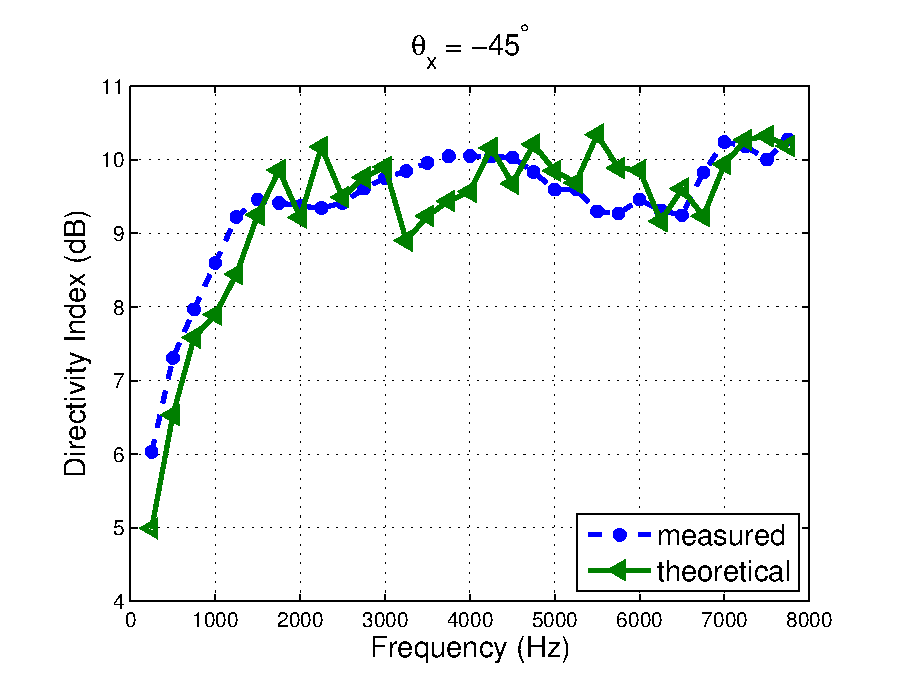
\includegraphics[width=4.46cm]{DIcomp-45} \hspace{-0.4cm} \vspace{0.1cm}
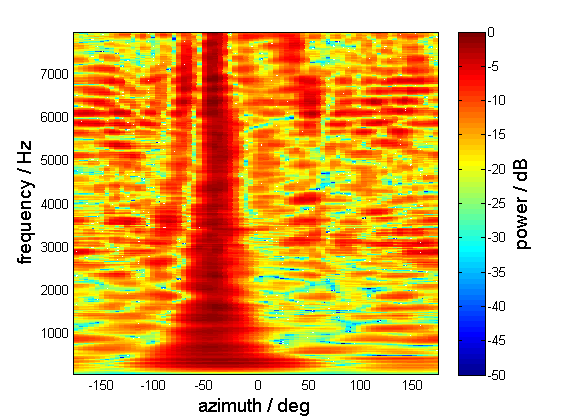
\includegraphics[width=4.46cm]{beam_-45}
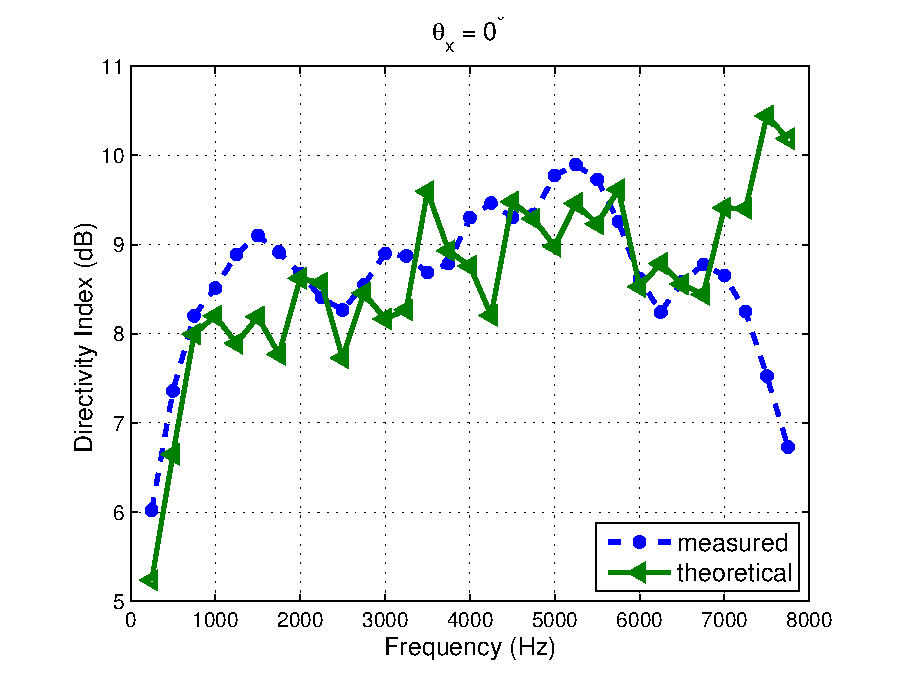
\includegraphics[width=4.46cm]{DIcomp0} \hspace{-0.4cm} \vspace{0.1cm}
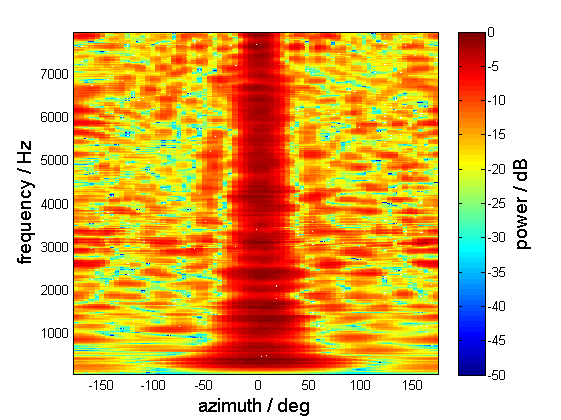
\includegraphics[width=4.46cm]{beam0}
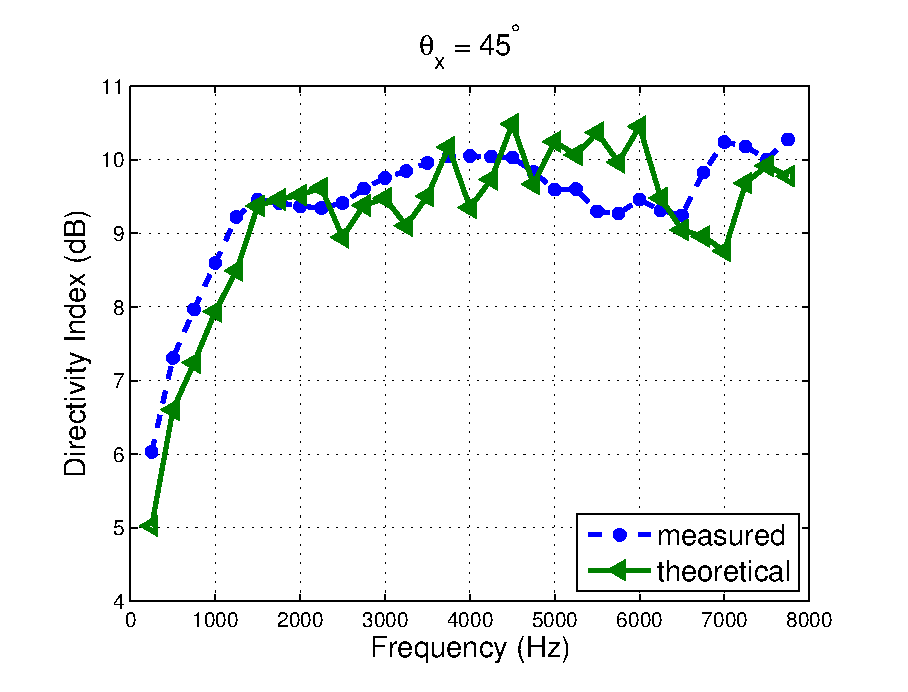
\includegraphics[width=4.46cm]{DIcomp45} \hspace{-0.4cm} \vspace{0.1cm}
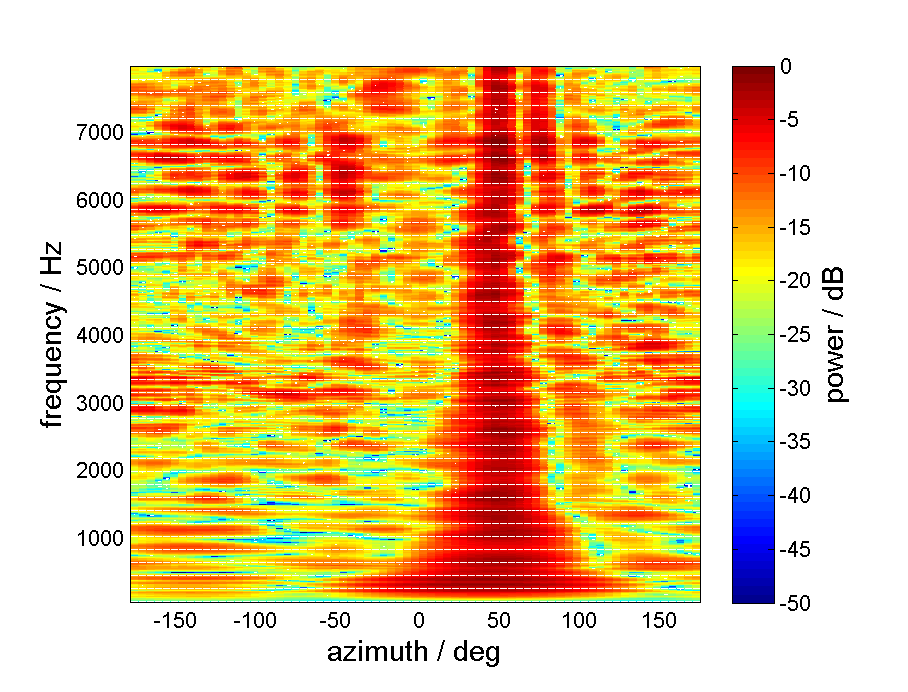
\includegraphics[width=4.46cm]{beam_45} \vspace{0.1cm}
\begin{minipage}[h]{0.25\textwidth}
\begin{center}
\small (a)
\end{center}
\end{minipage} \vspace{-0.4cm}
\begin{minipage}[h]{0.25\textwidth}
\begin{center}
\small (b)
\end{center}
\end{minipage} \vspace{-0.4cm} 
 \caption{(a) Theoretical and measured directivity index and (b) measured beam patterns of the optimal array configuration found through the sifting approach}\vspace{-0.2 cm}
\label{fig: dipatterns}
\end{figure}
%\begin{figure}[b!]
%\small
%\centering
%  \begin{minipage}[t]{.2\textwidth} 
%	  \begin{center}
%	  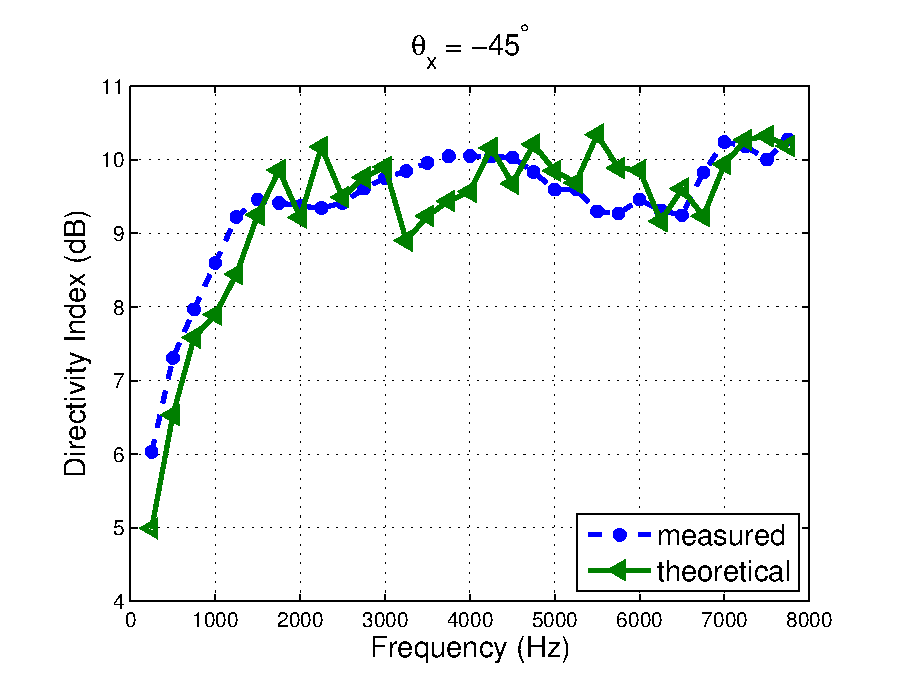
\includegraphics[scale=0.26]{DIcomp-45}
%	  \end{center}
%	  \end{minipage}
%	   \begin{minipage}[t]{.2\textwidth} 
%	  \begin{center}
%	  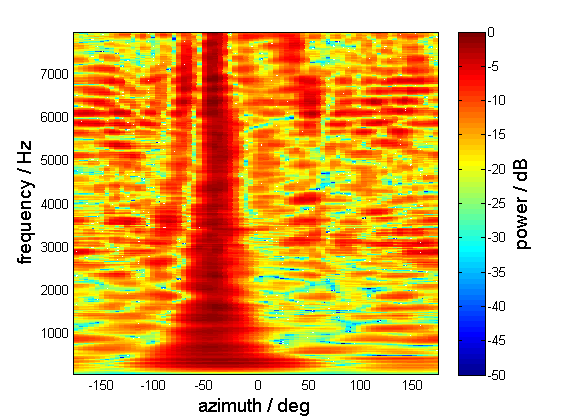
\includegraphics[scale=0.26]{beam_-45}
%	  \end{center}
%	  \end{minipage}
%	  \begin{minipage}[t]{.2\textwidth} 
%	  \begin{center}
%	  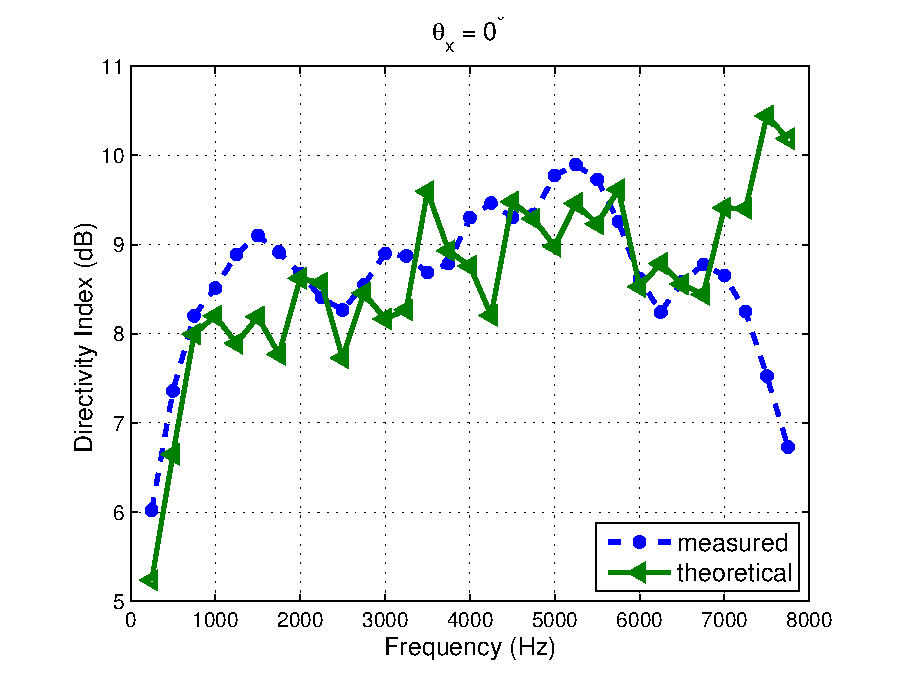
\includegraphics[scale=0.26]{DIcomp0}
%	  \end{center}
%	  \end{minipage}
%	   \begin{minipage}[t]{.2\textwidth} 
%	  \begin{center}
%	  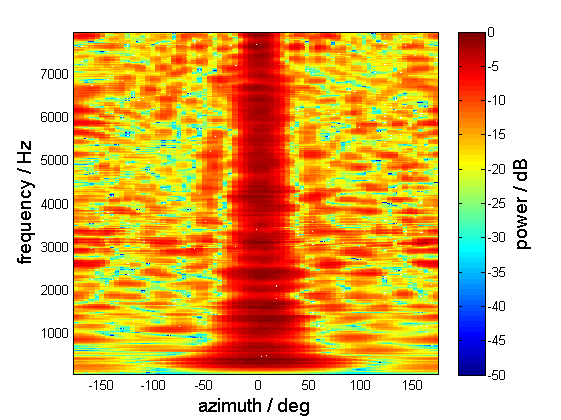
\includegraphics[scale=0.26]{beam0}
%	  \end{center}
%	  \end{minipage}
%	   \begin{minipage}[t]{.2\textwidth} 
%	  \begin{center}
%	  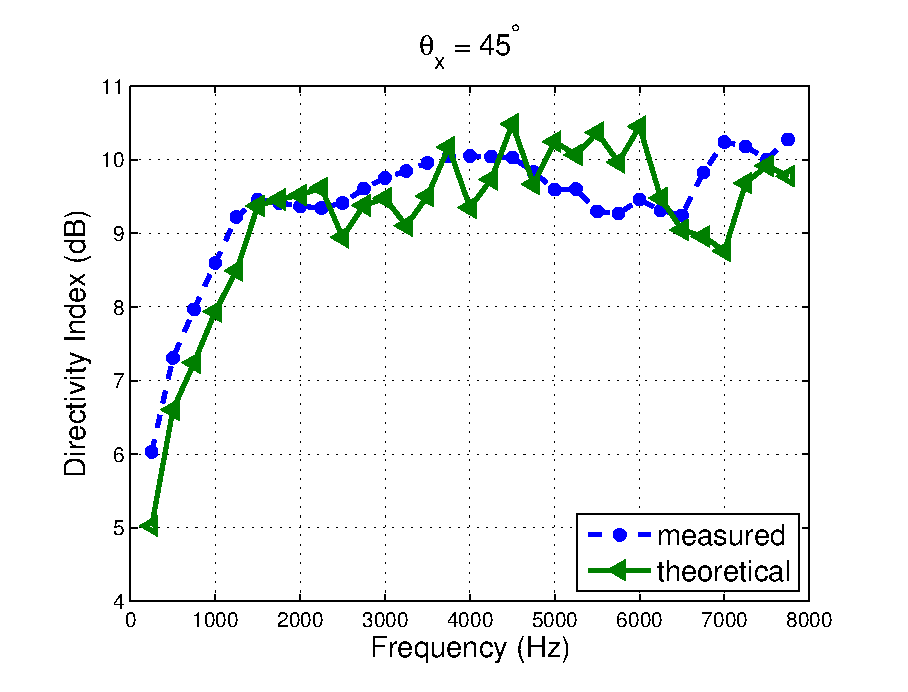
\includegraphics[scale=0.26]{DIcomp45}
%	  {\small (a)}
%	  \end{center}
%	  \end{minipage}
%	   \begin{minipage}[t]{.2\textwidth} 
%	  \begin{center}
%	  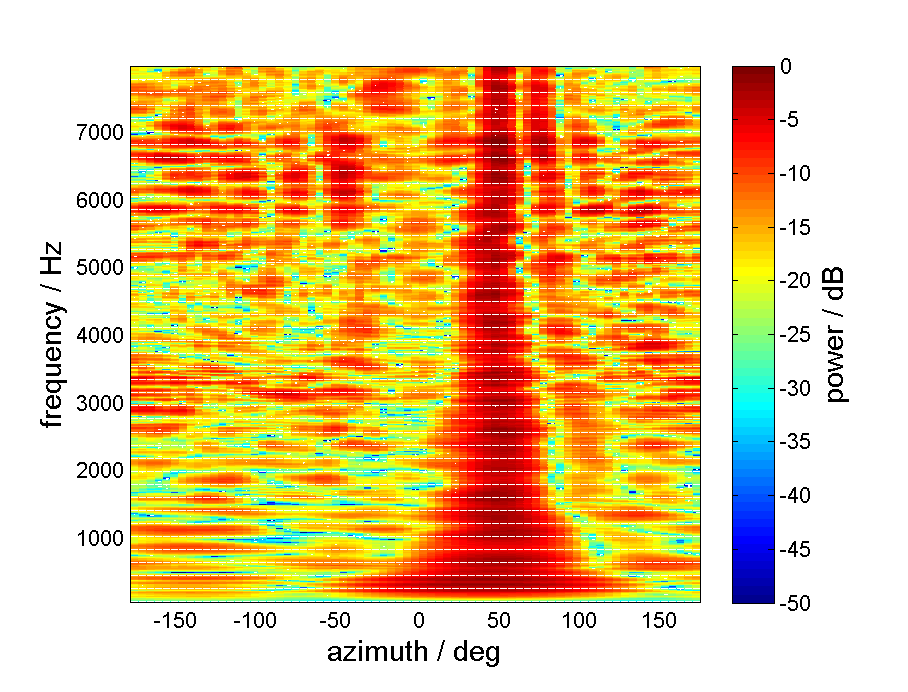
\includegraphics[scale=0.26]{beam_45}
%	  {\small (b)}
%	  \end{center}
%	  \end{minipage}
%	  \caption{Theoretical and measured directivity index (a) and measured beam patterns (b) of the optimal array configuration found through the sifting approach}
%	  \label{fig: dipatterns}
%	  \end{figure}
\vspace{-0.2cm}
\section{Conclusion}
\vspace{-0.2cm}
In this paper we have described several computationally efficient approaches for optimizing the microphone positions for planar superdirective beamformers, that are required to steer towards several angles. Through the derivation of an upper bound on the achievable performance, it is shown that the proposed methods find near-optimal configurations. Furthermore, we have demonstrated their usability for designing a superdirective beamformer using $8$ microphones to steer towards $3$ steering angles.


\begin{thebibliography}{10}

\bibitem{MAbook2}
J.~Bitzer and K.~U. Simmer,
\newblock ``Superdirective microphone arrays,''
\newblock in {\em Microphone Arrays: Signal Processing Techniques and
  Applications}, chapter~2, pp. 19--37. Springer Verlag, 2001.
\vspace{-0.45cm}
\bibitem{Elkobook}
G.~Elko,
\newblock ``Superdirectional microphone arrays,''
\newblock in {\em Acoustic Signal Processing for Telecommunication},
  chapter~10, pp. 181--237. Kluwer Academic Publishers, Boston, 2000.
\vspace{-0.05cm}
\bibitem{kajala_broadband_99}
M.~Kajala and M.~H\"am\"al\"ainen,
\newblock ``Broadband beamforming optimization for speech enhancement in noisy
  environments,''
\newblock in {\em Proc. IEEE Workshop on Applications of Signal Processing to
  Audio and Acoustics}, New Paltz, NY, Oct. 1999, pp. 19--22.
\vspace{-0.05cm}
\bibitem{ITG}
S.~Gergen, N.~Madhu, and R.~Martin,
\newblock ``A new performance criterion for microphone array geometries and
  filter-and-sum beamforming,''
\newblock in {\em Proc. ITG Conference on Speech Communication}, Bochum,
  Germany, Oct. 2010.
\vspace{-0.05cm}
\bibitem{Goodwin_optimization_2005}
M.~M. Goodwin,
\newblock ``Cost-constrained broadband array design based on optimal spacing,''
\newblock in {\em Proc. IEEE Workshop on Applications of Signal Processing to
  Audio and Acoustics}, New Paltz, NY, Oct. 2005, pp. 98--101.
\vspace{-0.05cm}
\bibitem{planar}
R.~Martin, A.~Petrovsky, and T.~Lotter,
\newblock ``Planar superdirective microphone arrays for speech acquisition in
  the car,''
\newblock in {\em Proc. European Conference on Speech Communication and
  Technology}, Aalborg, Denmark, Sep. 2001, pp. 2623--2626.
\vspace{-0.05cm}
\bibitem{doclomoonensd}
S.~Doclo and M.~Moonen,
\newblock ``Superdirective beamforming robust against microphone mismatch,''
\newblock {\em IEEE Trans. Audio, Speech, Language Processing},
  vol. 15, no. 2, pp. 617--631, Feb. 2007.
\vspace{-0.05cm}
\bibitem{skolnik_dynamic_64}
M.~I. Skolnik, G.~Nemhauser, and J.~W. Sherman,
\newblock ``Dynamic programming applied to unequally spaced arrays,''
\newblock {\em IEEE Trans. Antennas and Propagation}, vol. 12, no. 1,
  pp. 35--43, Jan. 1964.
\vspace*{-0.45cm}
\bibitem{GAbook}
C.~R. Reeves and J.~E. Rowe,
\newblock {\em Genetic algorithms - principles and perspectives}, chapter~2,
  pp. 19--60,
\newblock Kluwer Academic Publishers, Massachusetts, 2003.
\vspace{-0.05cm}
\bibitem{ANSI}
American National Standards Institute,
\newblock {\em American National Standard Specification for Octave-Band and
  Fractional-Octave-Band Analog and Digital Filters}, 1986.
\vspace{-0.05cm}
\end{thebibliography}

\end{document}